\lecture{20}{2025-04-30}{The rate}{}

\begin{parag}{Code $\mathcal{C}$}
    Let use have the code $\mathcal{C}$:
    \begin{minipage}{0.5\textwidth}
    \begin{align*} 0000\\0011\\1100\\1111 \end{align*}
    \end{minipage}
    \begin{minipage}{0.5\textwidth}
    We want to find $n, k, $ rate and $d_{min}$.
    \begin{itemize}
        \item $n = 4$
        \item $k = \log_2 \left|\mathcal{C}\right| = \log_2 4 = 2$
        \item rate: $\frac{2}{4} = \frac{1}{2}$
        \item $d_{min} = 2$
    \end{itemize}
\end{minipage} 

    If we take the code:
    \begin{minipage}{0.5\textwidth}
    \begin{align*} 0000\\ 1111 \end{align*}
    \end{minipage}
    \begin{minipage}{0.5\textwidth}
    \begin{itemize}
        \item $n = 4$
        \item $k = \log_2 \left|\mathcal{C}\right| = \log_2 2 = 1$
        \item rate: $\frac{1}{4} = \frac{1}{4}$
        \item $d_{min} = 4$
    \end{itemize}
\end{minipage} 
 
    For example without binary code:
    \begin{minipage}{0.5\textwidth}
    \begin{align*} 000\\001\\002\\ \vdots\\ 222 \end{align*}
    \end{minipage}
    \begin{minipage}{0.5\textwidth}
    \begin{itemize}
        \item $n = 3$
        \item $k = \log_2 \left|\mathcal{C}\right| = \log_2 27 $
        \item rate: $\frac{\log_2 27}{3} = \frac{\text{bits}}{\text{channel use}}$ which is the thing you get when you ask swisscom how much 4g you have.
\\ If we take for example a better universe: 
\begin{align*} k = \log_3 \left|\mathcal{C}\right| = \log_3 27 = 3
\end{align*}
\begin{align*} \text{rate} =  \frac{k}{n} = \frac{3}{3} =  1 \end{align*}
        \item $d_{min} = 1$
    \end{itemize}
 
\end{minipage} 
    
But we can take the alphabet in a smart way:
\begin{minpage}{0.5\textwidth}
    \begin{align*} 000\\011\\022\\110\\220\\121\\102\\201\\212 \end{align*}
\end{minpage}
    \begin{minipage}{0.5\textwidth}
     \begin{itemize}
        \item $n = 3$
        \item $k = \log_3 \left|\mathcal{C}\right| = \log_3 9 = 2$
        \item rate: $\frac{k}{n} = \frac{2}{3}$
        \item $d_{min} = 2$
    \end{itemize}
    \end{minipage}
\end{parag}


\begin{parag}{Erasure correction: how it relates to $d_{min}\left(\mathcal{C}\right)$}
    \begin{theoreme}
        A minimum-distance decoder for a code $\mathcal{C}$ \important{corrects} (fill in) \important{all the erasures} of weight $p$ if and only if $p < d_{min}\left(\mathcal{C}\right)$
    \end{theoreme}
    Let us do it for the previous code (the one right before).\\
    If we take for example $220 \to $ ERASURE $\to 2?2$ the claim now is the we actually can recover from this. Let us check the alphabet which one has a $2$ one the first side and a $0$ on the other side. We check and we see that there is only one in the alphabet that check all the ticks: 220. We can also say we chose the one that has the smallest hamming distance with the erased codeword.
\end{parag}
\begin{parag}{Proof $\impliedby$}
    Suppose that $ p < d_{min}\left(\mathcal{C}\right)$.\\
    Let $c$ and $ y $ be the input and the output of an erasure channel, respectively, with $d\left(c, y\right) = p$.\\
    We show that there is only one way to fille in the erased positions.\\
    let $c \in \mathcal{C}$ and $\overline{c} \in \mathcal{C}$ be two codewords that agree with $y$ in the non-erased positions.\\
    Clearly, $d\left(c, \overline{c}\right) \leq p < d_{min}\left(\mathcal{C}\right)$ This is possible only if $c = \overline{c}$.
\end{parag}
\begin{parag}{Proof $\implies$}
    We use contraposition.\\
    Suppose that $p= d_{min}\left(\mathcal{C}\right)$\\
    We construct an example where the decoder will not always decode correctly.\\
    Let $c$ and $c'$ be codewords at distance $d_{min}\left(\mathcal{C}\right)$.\\
    Let $c$ be the channel input, and suppose
    
    \begin{subparag}{Illustrative example}
        given the alphabet
        \begin{align*} 0000\\0011\\1100\\1111 \end{align*}
        You can see that if you take the erased $00??$ you cannot know which one is it is. we took here the $p = d_{min}\left(\mathcal{C}\right)$ and as you can see we cannot guess.
        
    \end{subparag}
\end{parag}
\begin{parag}{Error correction}
    \begin{theoreme}
        A minimum-distance decoder for a code $\mathcal{C}$ \important{corrects all channel errors} of weight $p$ if and only if $p < \frac{d_{min}\left(\mathcal{C}\right)}{2}$.
    \end{theoreme}
    
\end{parag}
\begin{parag}{Proof}
    Let have the true codeword $C$, noisy channel output $y$. Given the assumption, $d\left(c, y\right) = p$. Let $\overline{c}$ be the output of the minimum distance decoder. Therefore if we want to comput the hamming distance between $\overline{c}$ and $y$ we get:
    
    \begin{align*} d\left(\overline{c}, y\right) \leq p \end{align*}
    Then by the triangle inequality: 
    \begin{align*} d\left(c, \overline{c}\right) &\leq d\left(c, y\right) + d\left(y, \overline{c}\right) \\
    &\leq 2p < d_{min}\left(\mathcal{C}\right)
    \end{align*}
    Hence, $c =  \overline{c}$  \\
    Hence, the minimum distance decoder output the correct answer.
    
    A finir la preuve
    
\end{parag}
\begin{parag}{Summary}
   \begin{center}
   \begin{tabular}{c|c|c}
    & detection guaranteed if  & correction guaranteed if \\
    \hline
       erasure channel & (not applicable) & $p < d_{min}$  \\
       \hline
       error channel & $p < d_{min}$ & p < $\frac{d_{min}}{2}$
   \end{tabular}
   \end{center}
    
    
\end{parag}


\begin{parag}{Upper bound to $d_{min}\left(\mathcal{C}\right)$}
    Recall the important parameters of a block code $\mathcal{C}$ over a D-ary alphabet:
    \begin{itemize}
        \item $n$, the block length
        \item $k =  \log_D \left|\mathcal{C}\right|$ the number of information symbols carried by a codeword. (Equivalently, $\mathcal{C} = D^k$)
    \end{itemize}

\end{parag}
\begin{parag}{Singleton's bound}
    

    \begin{theoreme}
    Refardless of the alphabet size, the minimum distance of a block code satisfies:
    \begin{align*} d_{min} - 1 \leq n-k \end{align*}
    \end{theoreme}
    Block codes that satisfy the singleton bound with equality are called \important{Maximum distance separable} codes. (\important{MDS} codes).
\end{parag}
\begin{parag}{Proof}
    \begin{center}
    \begin{tabular}{|c|c|c|c|c|c|}
        & 1 & 2 & 3 & $\ldots$ & n \\
        \hline
        1 & 0 & 5 & 1 &$\ldots$ & 0 \\
        \hline
        2 & 2 & 1 & 2 & $\ldots$ & 3  \\
        $\vdots$ \\
        \hline
        $D^k$ &  9 & 0 & 2 & $\ldots$ & 2
    \end{tabular}
    \end{center}
    You can then get rid of the $d_{min} - 1$ from the right like this:
    \begin{center}
        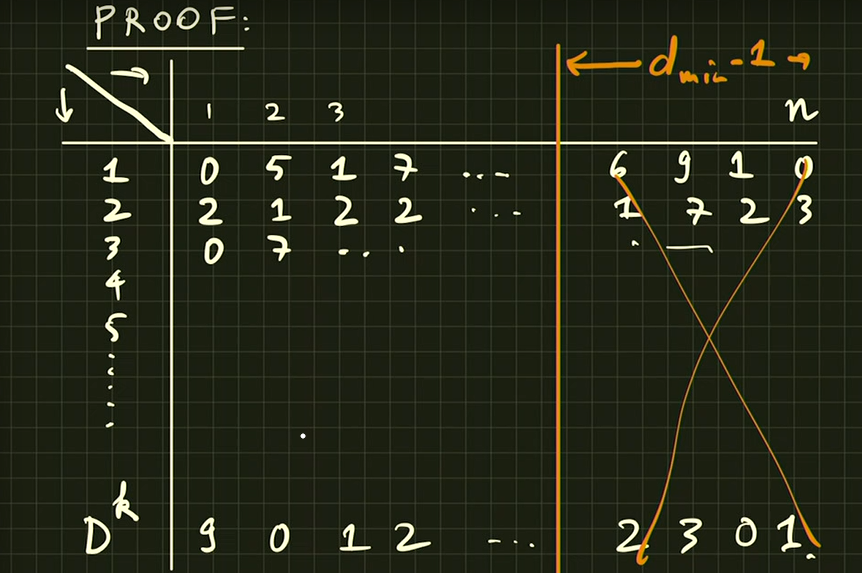
\includegraphics[scale=0.3]{22025-04-30.png}
    \end{center}
    The next question after this is: how many different strings of length $n- \left(d_{min} - 1\right)$ can we have?\\
    We can you combination with the alphabet cardinilality being $D$ we get:
    \begin{align*} nbr_{comb} = D^{n - \left(d_{min} - 1\right)} \end{align*}
    Hence we must have:
    \begin{align*} D^k \leq D^{n-\left(d_{min}-1\right)} \end{align*}
    
    
    \begin{subparag}{Remark}
        \begin{framedremark}
            here $k$ doesn't have to be a integer, only $D^k$ \textbf{has to } be an integer (by assumption) 
        \end{framedremark}
        
        
    \end{subparag} 
\end{parag}

\begin{parag}{Pigeonhole principle}
   a lire mais pas vu en cours donc voila  (``it is a bit overkill'')
\end{parag}
\begin{parag}{Exercise}

    
\end{parag}








